% Options for packages loaded elsewhere
\PassOptionsToPackage{unicode}{hyperref}
\PassOptionsToPackage{hyphens}{url}
%
\documentclass[
]{article}
\usepackage{lmodern}
\usepackage{amssymb,amsmath}
\usepackage{ifxetex,ifluatex}
\ifnum 0\ifxetex 1\fi\ifluatex 1\fi=0 % if pdftex
  \usepackage[T1]{fontenc}
  \usepackage[utf8]{inputenc}
  \usepackage{textcomp} % provide euro and other symbols
\else % if luatex or xetex
  \usepackage{unicode-math}
  \defaultfontfeatures{Scale=MatchLowercase}
  \defaultfontfeatures[\rmfamily]{Ligatures=TeX,Scale=1}
\fi
% Use upquote if available, for straight quotes in verbatim environments
\IfFileExists{upquote.sty}{\usepackage{upquote}}{}
\IfFileExists{microtype.sty}{% use microtype if available
  \usepackage[]{microtype}
  \UseMicrotypeSet[protrusion]{basicmath} % disable protrusion for tt fonts
}{}
\makeatletter
\@ifundefined{KOMAClassName}{% if non-KOMA class
  \IfFileExists{parskip.sty}{%
    \usepackage{parskip}
  }{% else
    \setlength{\parindent}{0pt}
    \setlength{\parskip}{6pt plus 2pt minus 1pt}}
}{% if KOMA class
  \KOMAoptions{parskip=half}}
\makeatother
\usepackage{xcolor}
\IfFileExists{xurl.sty}{\usepackage{xurl}}{} % add URL line breaks if available
\IfFileExists{bookmark.sty}{\usepackage{bookmark}}{\usepackage{hyperref}}
\hypersetup{
  hidelinks,
  pdfcreator={LaTeX via pandoc}}
\urlstyle{same} % disable monospaced font for URLs
\usepackage[margin=1in]{geometry}
\usepackage{graphicx,grffile}
\makeatletter
\def\maxwidth{\ifdim\Gin@nat@width>\linewidth\linewidth\else\Gin@nat@width\fi}
\def\maxheight{\ifdim\Gin@nat@height>\textheight\textheight\else\Gin@nat@height\fi}
\makeatother
% Scale images if necessary, so that they will not overflow the page
% margins by default, and it is still possible to overwrite the defaults
% using explicit options in \includegraphics[width, height, ...]{}
\setkeys{Gin}{width=\maxwidth,height=\maxheight,keepaspectratio}
% Set default figure placement to htbp
\makeatletter
\def\fps@figure{htbp}
\makeatother
\setlength{\emergencystretch}{3em} % prevent overfull lines
\providecommand{\tightlist}{%
  \setlength{\itemsep}{0pt}\setlength{\parskip}{0pt}}
\setcounter{secnumdepth}{-\maxdimen} % remove section numbering

\author{}
\date{\vspace{-2.5em}}

\begin{document}

\doublespacing

\section{Introduction}
\label{sec4:Introduction}

Many of the ideas and concepts {[}@dobson2008introduction{]} of linear
regression modelling carry over to generalized regression modelling,
however the ``generalized'' term is used to refer to all linear models
other than simple straight lines found in the linear case. That is, the
generalized linear regression (GLR) model reduces (multiple) linear
regression (MLR) if and only if the error term (random component of the
response variable \(y\)) has a normal distribution i.e., \(\mu = 0\), \&
\(\sigma^2\):

\singlespacing

\begin{eqnarray}\label{linearmodel}
E(\mathbf{Y_i}) = \mathbf{\mu_i} = \mathbf{x_i}^T\mathbf{\beta} + \epsilon_i \qquad \epsilon_i \thicksim \mathbf{N(0, \sigma^2)},
\end{eqnarray} \doublespacing

In the case of the OpRisk dataset, the relationship between outcomes and
drivers of risk are frequently not normal, therefore models of the form
\ref{linearmodel} where random variables \(\mathbf{Y_i}\) are
independent, are not applicable. The transposed vector
\(\mathbf{x_i}^T\) represents the \(i\)th row of the dataset
\(\mathbf{X}\). In such cases, due to recent advances in statistical
theory and computational techniques, generalised linear models (GLM);
which are analogous to linear models, are used to assess and quantify
the relationships between a target variable and explanatory variables
{[}@dobson2008introduction{]}.\medskip

GLM's differ in that

\begin{itemize}
\item The distribution of the target variable is chosen from the exponential family
\item A transformation of the mean of the response is linearly related to the explanatory variables, however their association need not be of the simple linear form in equation \ref{linearmodel}
\end{itemize}
\medskip

\section{Generalized linear (regression) models (GLM) for count data}
\label{sec4:Generalized linear (regression) models (GLM) for count data}

As with the linear model, consider independent rv's \(\mathbf{Y_i}\) not
i.i.d, whose probability depends on a parameter \(\theta_i\). The choice
of parameter \(\theta_i\) determines the response distribution which is
assumed to have the same form as the exponential family, in turn
characterising the statistical unit \(i\). Thus, the exponential family
representation depends on varying parameters \(\theta_i\), and a
constant scale parameter \(\phi\). the pdf of \(\mathbf{Y_i}\) is

\singlespacing

\begin{eqnarray}\label{Exponentialfamily}
f(y_i;\theta_i;\phi) = \exp\left[\frac{a(y_i)b(\theta_i) -c(\theta_i)}{\phi}-d(y_i,\phi)\right], \quad y_i \in Y 
\end{eqnarray} \doublespacing

where \(a\), \(b\), \(c\), \& \(d\) are regarded as known functions.
Expanding the expression in equation \ref{Exponentialfamily} yields

\singlespacing

\begin{eqnarray}\label{Exponentialfamilies}
f(y_i;\theta_i;\phi) &=& \exp\left[\frac{a(y_i)b(\theta_i) -c(\theta_i)}{\phi}-d(y_i,\phi)\right] \nonumber\\
 &=& \frac{1}{e^{d(y,\phi)}}\exp\left[\frac{a(y_i)b(\theta_i) -c(\theta_i)}{\phi}\right] \nonumber\\
 &=& r(y,\phi)\frac{1}{e^{\frac{c(\theta_i)}{\phi}}}\exp\left[\frac{a(y_i)b(\theta_i)}{\phi}\right] \nonumber\\
 &=& r(y,\phi)s(\theta,\phi)\exp\left[\frac{a(y_i)b(\theta_i)}{\phi}\right]\\
 \mbox{where} \quad r(y,\phi) &=& \frac{1}{e^{d(y,\phi)}}\quad \mbox{and where}\quad s(\theta,\phi) = \frac{1}{e^{\frac{c(\theta_i)}{\phi}}}\nonumber
\end{eqnarray} \doublespacing

since the scale parameter \(\phi\) is constant, the distribution belongs
to the exponential family if it can be written in the form

\singlespacing

\begin{eqnarray}\label{Exponential}
f(y;\theta) = r(y)s(\theta)\mathbf{e}^{a(y)b(\theta)}
\end{eqnarray} \doublespacing

If \(a(y) = y\), the distribution is in canonical form and \(b(\theta)\)
is called the natural parameter of the response distribution
{[}@de2008generalized{]}. The specific elements of a GLM are
{[}@dobson2008introduction; @covrig2015using{]}:

\begin{enumerate}
\item The random component given by the independent random variables $Y_1, Y_2, \ldots, Y_n $ not identically distributed. Note that the rv's $\mathbf{Y_i}$ for the Oprisk data, indexed by the subscript $i$, have different expected values $\mu_i$. Sometimes there may be only one observation $y_i$ for each $Y_i$, but there may be several observations $y_{ij}, (j=1,\ldots,n_i)$ for each $\mathbf{Y_i}$. The pdf or probability mass function of $\mathbf{Y_i}$ is given in equation \ref{Exponential} for $f(y)$, which specifies that the distribution of the response is in the exponential family. The support set $X$ of the rv $Y_i$ is subset of $\mathbf{N}$ of $\mathbf{R}$. 

\item The second advance is the extension of computational methods to estimate the models systematic component, so called the "linear predictor" described in equation \ref{linearmodel} built with $p+1$ parameters $\mathbf{\beta} = (\beta_0,\beta_1,\ldots,\beta_p)$ and with $p$ explanatory variables:

\singlespacing
\begin{eqnarray}\label{linearpredictor}
\eta_i = \beta_0 + \sum_{j=1}^{p}\beta_jx_{ij}, \qquad i = 1,2,\ldots,n
\end{eqnarray}
\doublespacing

\item The equation for $\eta_i$ specifies to the situation that there is some non-linear function, a transformation of the mean, $g(\mu)$, that is linearly related to the explanatory variables contained on the r.h.s of equation \ref{linearpredictor}, $\mathbf{X_i}^T\mathbf{\beta}$, i.e.,

\singlespacing
\begin{eqnarray}
g(\mu_i) = \mathbf{X_i}^T\mathbf{\beta}
\end{eqnarray}
\doublespacing

The function $g(\mu_i)$ is called the link function.
\end{enumerate}

\subsection{Interpretation}

Given a response variable \(y\), for the initial formulation of glm's by
@nelder1972generalized, \(b(\theta)\) determines the nature of the
response distribution and the choice of link is suggested by the
functional form of the relationship between the response and explanatory
variables. In choosing these components extra steps are taken compared
to ordinary regression modeling. Commonly used links functions are given
in Table \ref{tab_linkfcn} which also presents the units produced for
the various GLM links.

\begin{table}[tb]
\centering
\caption{The generalized linear model link functions with their associated units of interpretation. Note: This list is not exhaustive and there are likely more GLMs that are used within prevention research.} 
\label{tab_linkfcn}
\begin{tabular}{lcll}
\toprule
Link Function & $g(\mu)$ & Target variable Effect & Canonical link for \\ 
\midrule
Identity & $\mu$ & Original Continuous Unit & normal \\ 
  Log & ln$\mu$ & count & poisson \\ 
  Logit & ln $\frac{\mu}{1-\mu}$ & Risk & binomial \\ 
  Probit & $\phi^{-1}(\theta)$ & Risk & binomial \\ 
  Power & $\mu^p$ & Count & $\Gamma(p=-1)$\\
        &       & Count & inverse Gaussian(p=-2)\\
\bottomrule
\end{tabular}
\end{table}

\subsubsection{Offsets}

Modeling counts as realised operational hazard in an OpRisk group
requires correction for the period in days \(d\) exposed to risk. If
\(\mu\) is the mean of the count \(y\) then the occurence rate of
interest \(R= \frac{\mu}{d}\) and

\singlespacing

\begin{eqnarray}
g\left(\frac{\mu}{d}\right) = \mathbf{x}^T\mathbf{\beta}
\end{eqnarray} \doublespacing

When \(g\) is the log function, this becomes

\singlespacing

\begin{eqnarray}\label{offset}
\mbox{ln}\left(\frac{\mu}{d}\right) = \mathbf{x}^T\mathbf{\beta} \quad \Rightarrow \quad \mbox{ln}\mu = \mbox{ln}d + \mathbf{x}^T\mathbf{\beta}
\end{eqnarray} \doublespacing

Where the variable \(d\) appears representing the risk \emph{exposure}
and ln\(d\) is called an ``offset''. Equation \ref{offset} differs from
the usual specification of the linear predictor due to the inclusion of
the term ln\(d\). An offset is effectively another explanatory variable
in the regression, with a \(\beta\) coefficient = 1. With the offset,
\(y\) has expected value directly proportional to exposure:

\singlespacing

\begin{eqnarray}
E(Y) = \mu = d e^{x^T\beta}
\end{eqnarray} \doublespacing

Offsets are used to correct for differing periods of observation
{[}@de2008generalized{]} i.e., in the opRisk dataset these are the times
to detection (exposure) of the realised losses. The exposure measure is
a known constant which is readily incorporated into the estimation
procedure and is a quantity that is roughly proportional to the risk
{[}@parodi2014pricing{]} i.e., when the exposure (time to detection)
doubles whilst everthing else (e.g.~interest on an interest rate swap)
remains the same, the risk also doubles.

\section{Exploratory data analysis}
\label{sec:Exploratory data analysis}

The main source of the analysis dataset is primary data, a collection of
internal OpRisk losses for the period between 1 January 2013 and 31st
March 2013 at an investment bank in SA. The method of data generation
and collection is at the level of the individual trade deal, wherein
deal information is drawn directly from the trade generation and and
settlement system (TGSS) and edit detail from attribution reports
generated in middle office profit \& loss (MOPL). The raw source
consists of two separate datasets on a trade-by-trade basis of daily
frequencies (number of events) and associated loss severities.\medskip

The raw frequency data consists of 58,953 observations of 15 variables,
within the dataset there are 50,437 unique trades. The raw severity data
consists of 6,766 observations of 20 variables; within the severity
dataset there are 2,537 unique trades. The intersection between the
frequency and severity datasets consists of 2,330 individual
transactions which represent realised losses, pending and/or near
misses. This dataset is comprised of 3-month risk correction detail, in
the interval between 01 January 2013 and 31 March 2013. \medskip

\begin{table}[ht]
\centering
\caption{The contents of the traded transactions of the associated risk correction events.}
\begin{tabular}{lcc}
\toprule
  & \multicolumn{2}{c}{Storage} \\
Covariate     & Levels   & Type \\ 
\midrule
 Trade       &          & numeric \\
 UpdateTime  &          & numeric \\
 UpdatedDay  &          & numeric \\
 UpdatedTime &          & numeric \\
 TradeTime   &          & numeric \\
 TradedDay   &          & numeric \\
 TradedTime  &          & numeric \\
 Desk        &  10      & categorical \\
 CapturedBy  &  5       & categorical \\
 TradeStatus &  4       & categorical \\
 TraderId    &  7       & categorical \\
 Instrument  &  23      & categorical \\
 Reason      &  19      & categorical \\
 Loss        &          & numeric \\
 EventTypeCategoryLevel & 5  & categorical \\
 BusinessLineLevel      & 8  & categorical \\
 LossIndicator          & 2  & binary \\
 exposure               &    & numeric \\
 \bottomrule
\end{tabular}\label{tab_contents}
\end{table}

Two new variables are derived from the data; a target variable
(LossIndicator) is a binary variable whereupon, a \(1\) signifies a
realised loss, and \(0\) for those pending losses, or near misses. The
\emph{exposure} variable is computed by deducting the time between the
trade amendment (UpdateTime) and the time when the trade was booked
(TradeTime). It is a measure that is meant to be rougly proportional to
the risk of the transaction or a group of transactions. The idea is that
if the exposure (e.g.~the duration of a trade, the number of
allocation(trade splits), etc.) doubles whilst everything else (e.g.~the
rate, nominal of the splits, and others) remains the same, then the risk
also doubles.\medskip

In R, the GLM function works with two types of covariates/explanatory
variables: numeric (continuous) and categorical (factor) variables as
depicted in table \ref{tab_contents}. Multi-level categorical variables
are recoded by building dummy variables corresponding to each level.
This is achieved through an implemented algorithm in R, through a
transformation as recommended for the estimation of the GLM,
particularly in the estimation of the poisson regression model for count
data.\medskip

The model revolves around the fact that for each categorical variable
(covariate), previously transformed into a dummy variable, one must
specify a reference category from which the corresponding observations
under the same covariate are estimated and assigned a weight against in
the model {[}@covrig2015using{]}. By default in the GLM, the first level
of the categorical variable is taken as the reference level. As best
practice, @de2008generalized, @frees2010household, @denuit2007actuarial,
@cameron2013regression and others recommend that for each categorical
variable one should specify the modal class as the reference level; as
this variable corresponds to the level with the highes order of
predictability, excluding the dummy variable corrresponding to (weight
coefficient = \(e^0 = 1\)) the biggest absolute frequency.

\section{Description of the dataset}
\label{sec:Description of the dataset}

In this section, section \ref{sec:Description of the dataset}, the
dataset called \emph{OpRiskDataSet\_exposure}, provides data on the
increase in the numbers of operational events over a three month period,
beginning 01 January 2013 to end of 20 March 2013. For each transaction,
there is information about: trading risk exposure, trading
characteristics, causal factor characteristics and their cost.

\begin{figure}
\begin{subfigure}[b]{0.55\textwidth}
   \begin{frame}
      \centering
       \begin{tabular}{cc}
        Overall Loss Severity & Loss Severity as per Trading Role \\
        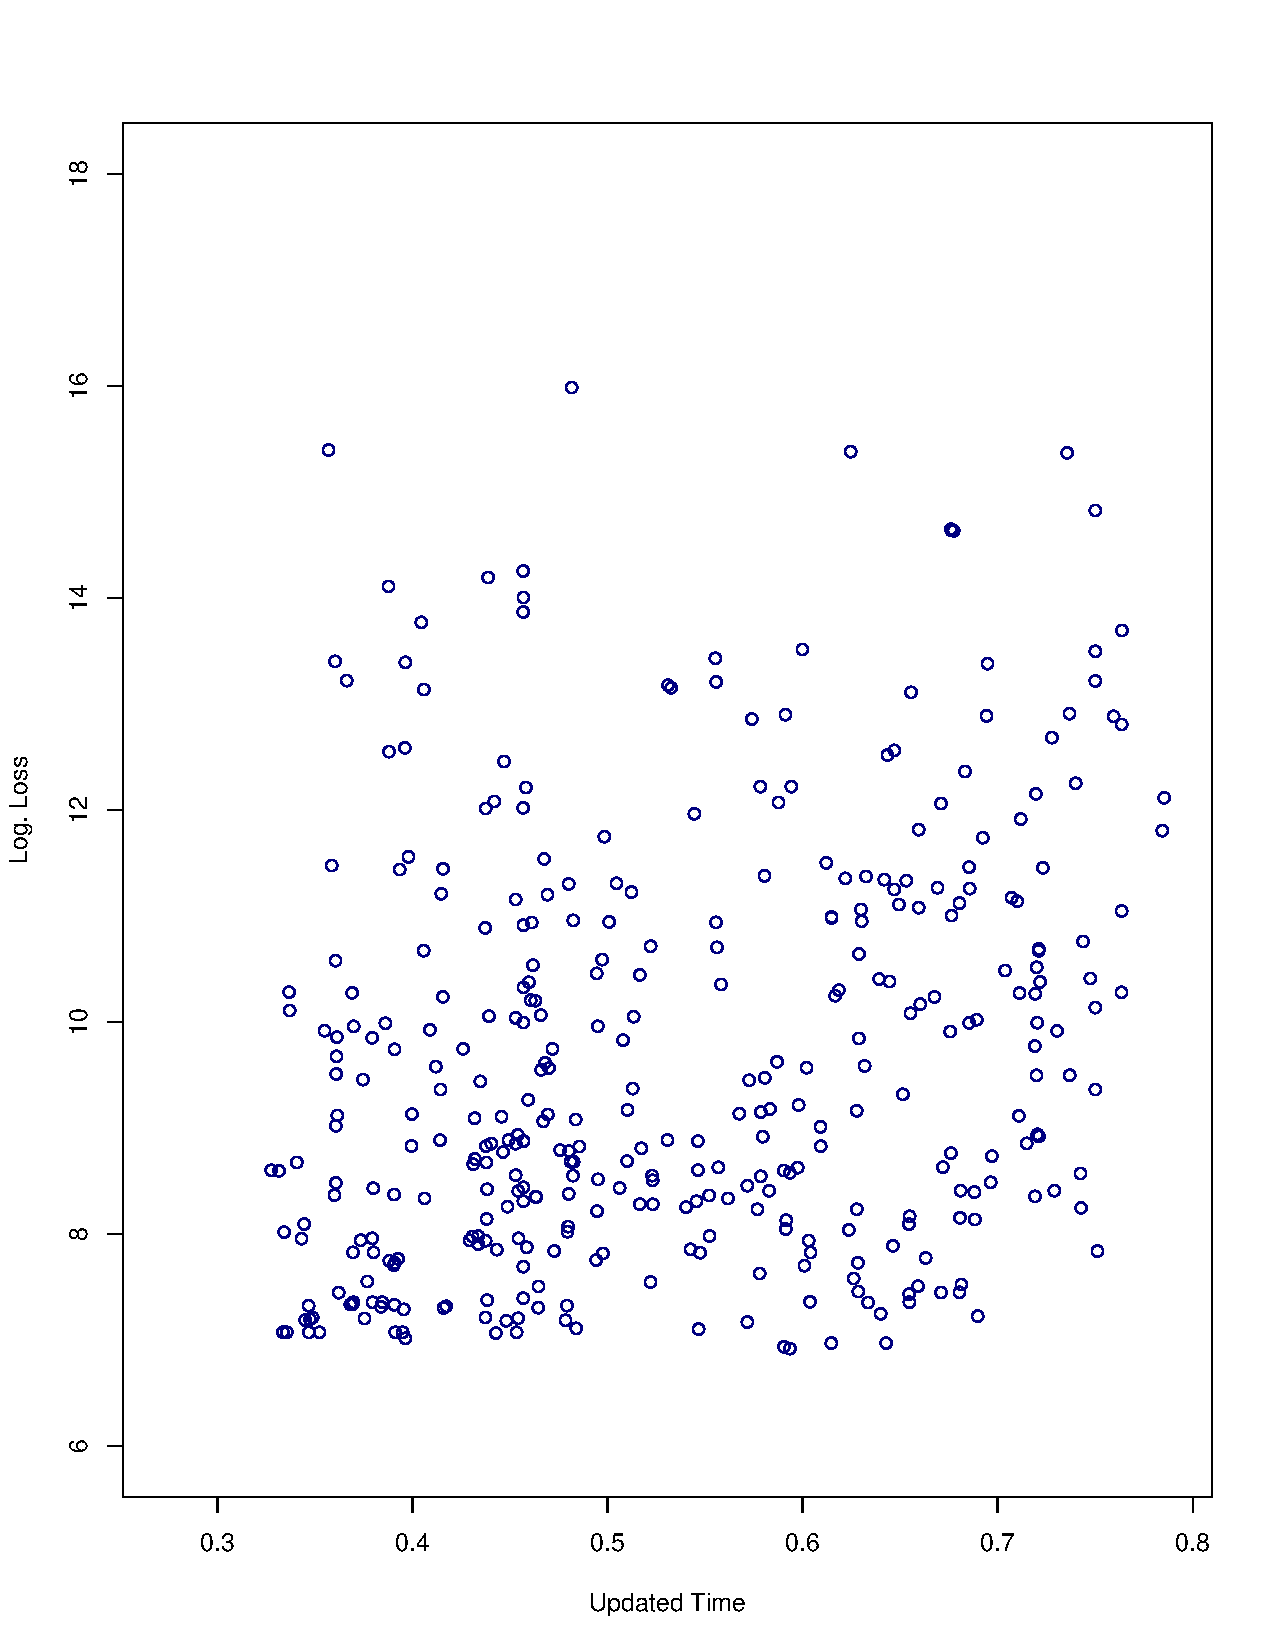
\includegraphics[height=5.5cm, width=7.5cm]{IntraDayUpdatedTime.pdf}
         &
         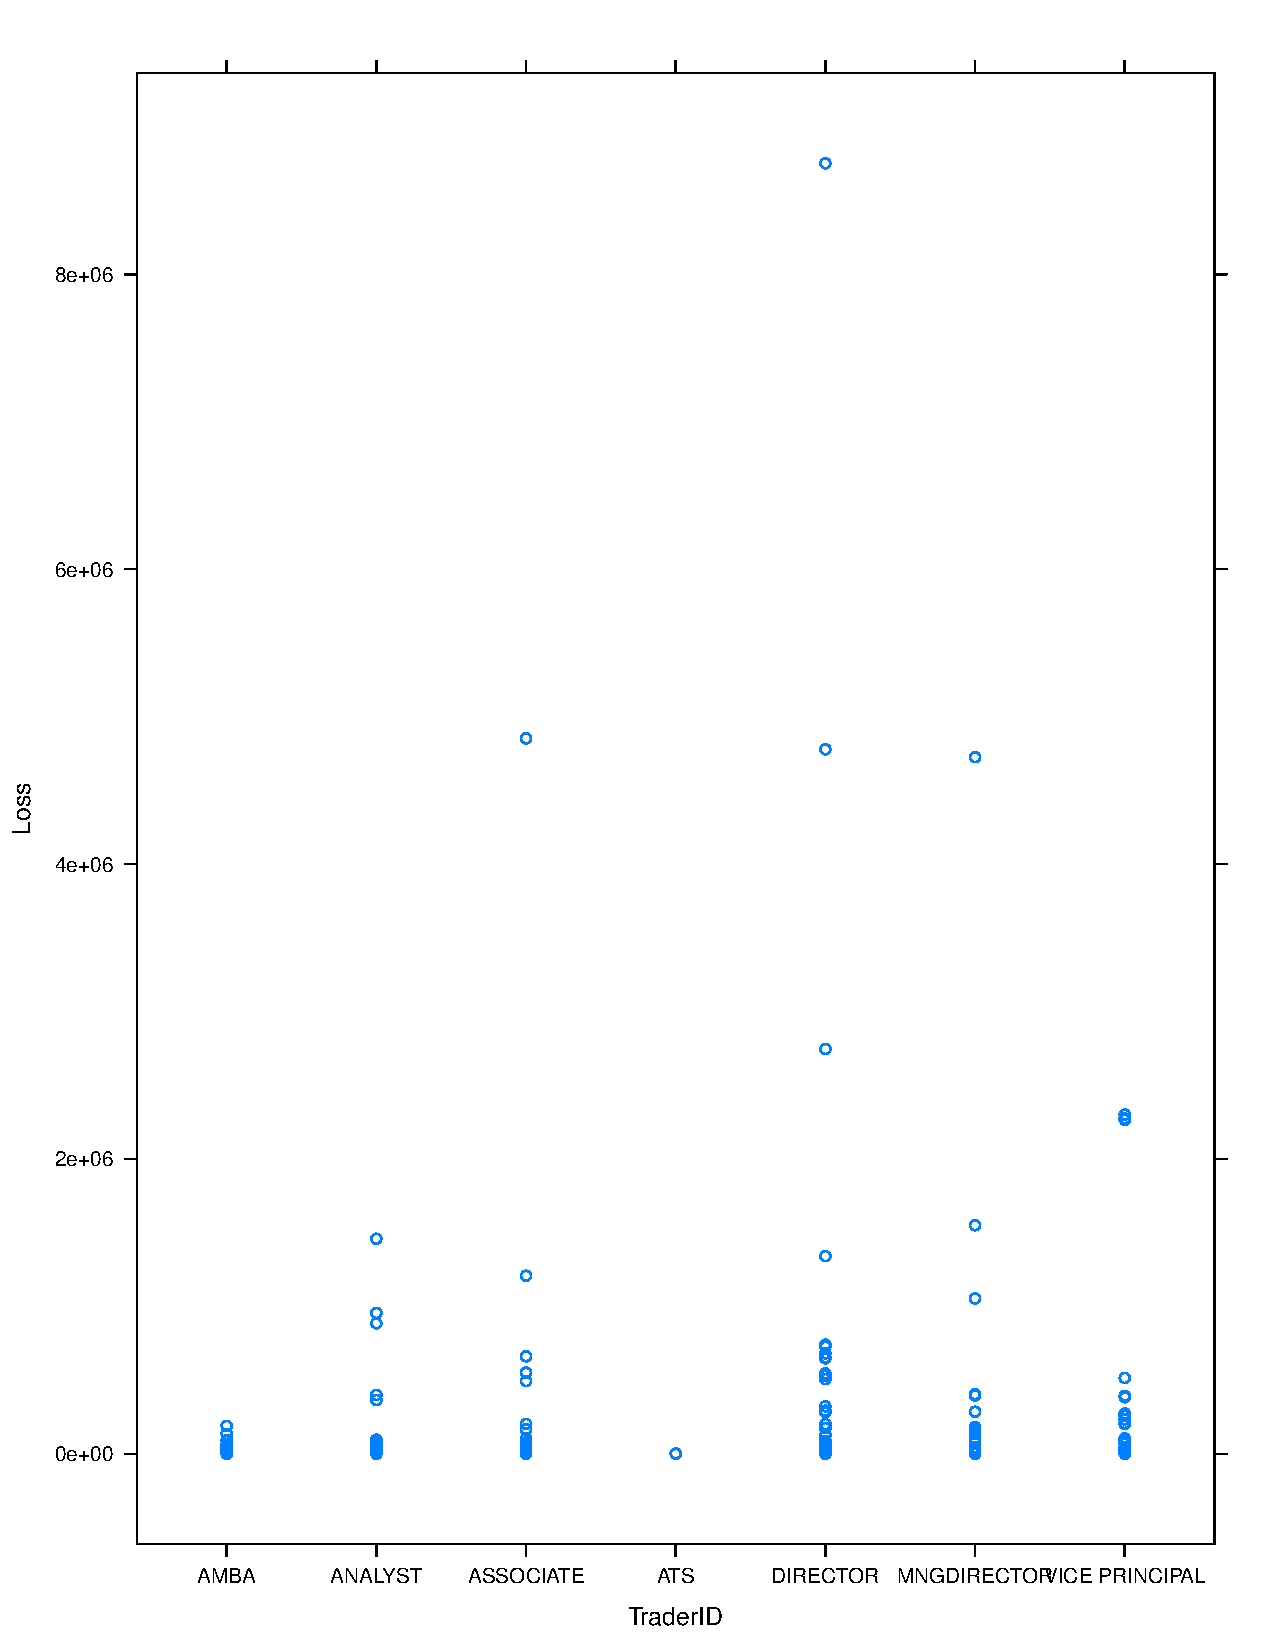
\includegraphics[height=5.0cm, width=7cm]{TrendTraderId.pdf}
         \end{tabular}
    \end{frame}
\subcaption{Intra-day trend analysis of loss severities: overall and as per trading role}
   \label{Intra_Day_Trends} 
\end{subfigure}

\begin{subfigure}[b]{0.55\textwidth}
   \begin{frame}
      \centering
       \begin{tabular}{cc}
        OpRisk events during month & Trading frequency \\
        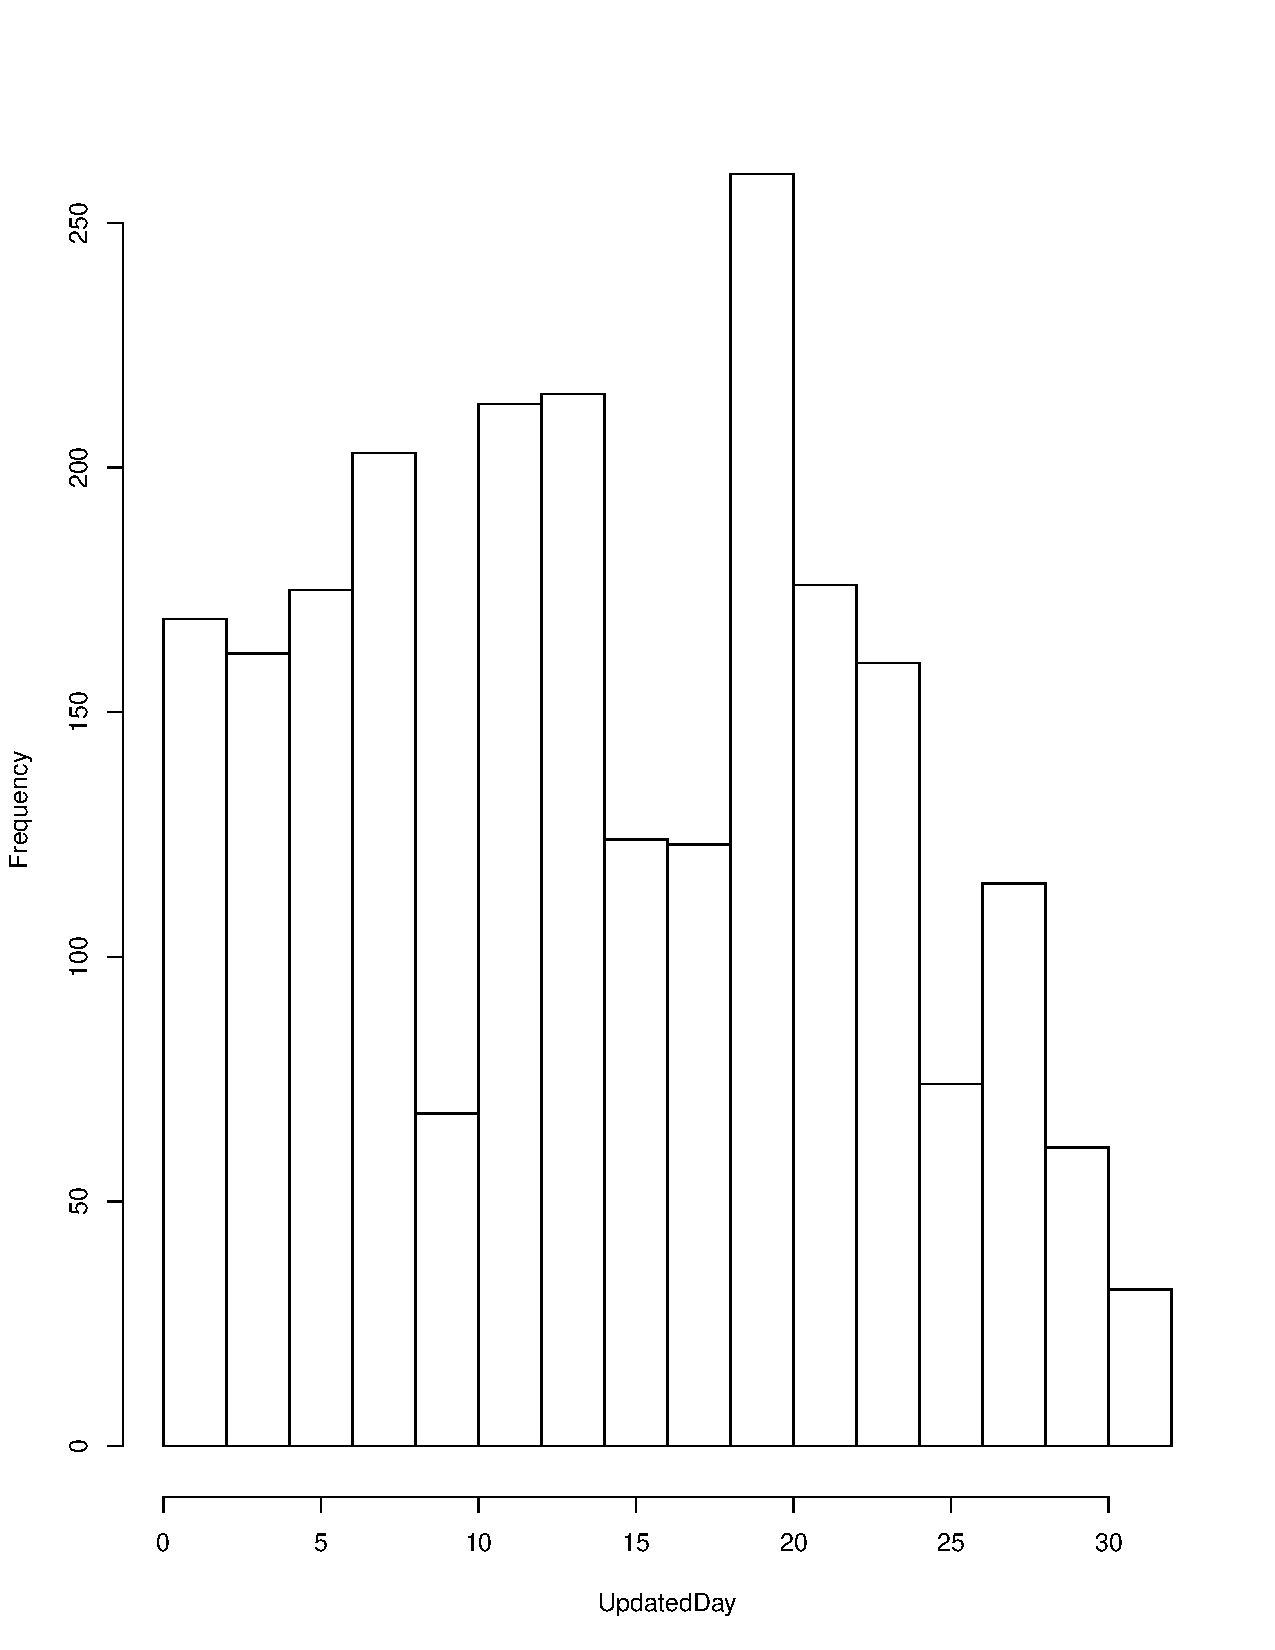
\includegraphics[height=5.5cm, width=7.5cm]{UpdatedDayFreq.pdf}
         &
         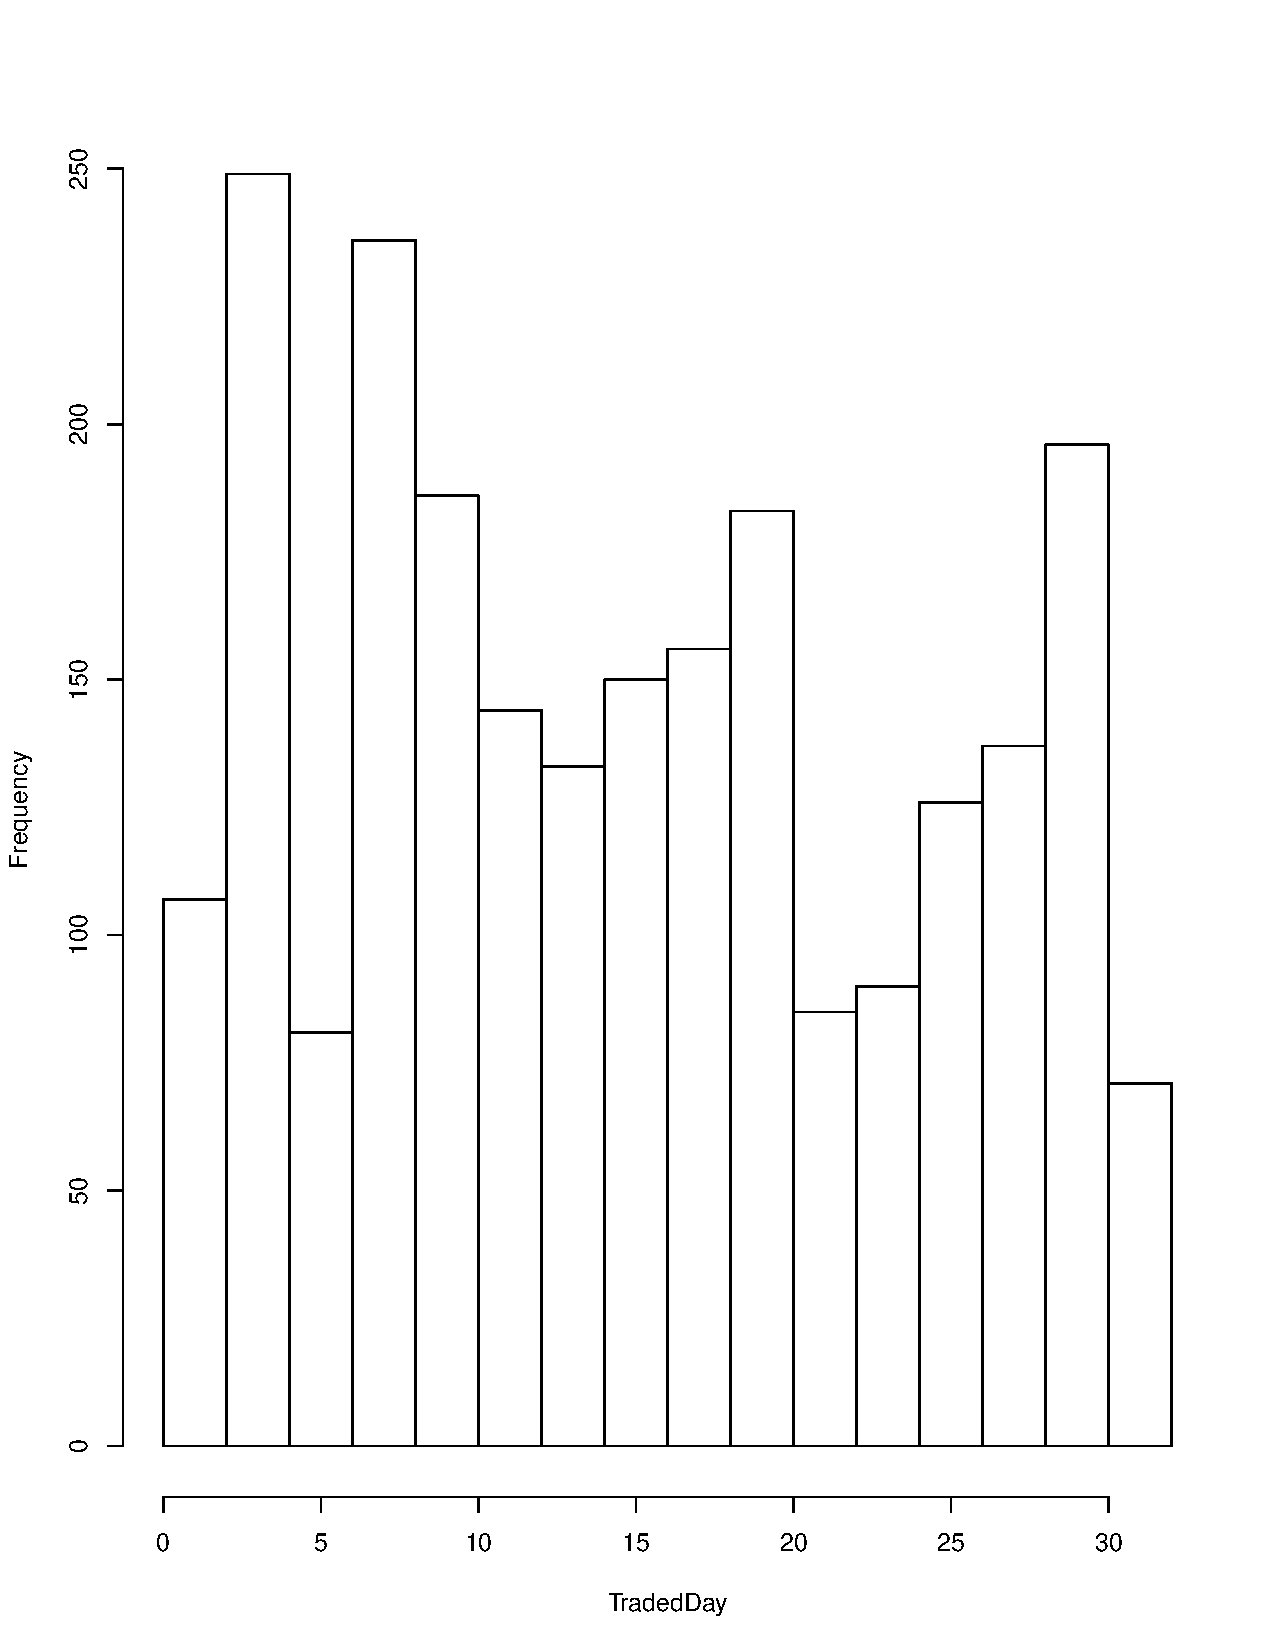
\includegraphics[height=5.5cm, width=7.5cm]{TradedDayFreq.pdf}
         \end{tabular}
    \end{frame}
\subcaption{Intra-month trends of OpRisk trading incidents compared to frequency of trading activity}
   \label{Hist_Loss_Freq}
\end{subfigure}
\caption[Numerical grid display]{(a) Scatterplots of intra-day trend analysis for logs of severities of operational events and for those identifying the trading role responsible/originating the loss incidents. (b) As for (a) but intra-month, and in the form of histograms depicting the frequency distrbution of the number daily operational indicents and the frequency of trades.} 
\end{figure}

\subsection{Characteristics of exposure}

\begin{verbatim}
## Rattle: A free graphical interface for data science with R.
## Version 5.3.0 Copyright (c) 2006-2018 Togaware Pty Ltd.
## Type 'rattle()' to shake, rattle, and roll your data.
\end{verbatim}

\begin{verbatim}
## 
## Attaching package: 'Hmisc'
\end{verbatim}

\begin{verbatim}
## The following objects are masked from 'package:base':
## 
##     format.pval, units
\end{verbatim}

\begin{verbatim}
## 
## Attaching package: 'dplyr'
\end{verbatim}

\begin{verbatim}
## The following objects are masked from 'package:Hmisc':
## 
##     src, summarize
\end{verbatim}

\begin{verbatim}
## The following objects are masked from 'package:stats':
## 
##     filter, lag
\end{verbatim}

\begin{verbatim}
## The following objects are masked from 'package:base':
## 
##     intersect, setdiff, setequal, union
\end{verbatim}

\begin{verbatim}
## 
## Attaching package: 'caret'
\end{verbatim}

\begin{verbatim}
## The following object is masked from 'package:survival':
## 
##     cluster
\end{verbatim}

The exposure of risk of type \(i\), \(d_i\) shows the daily duration,
from when the trade was booked to the moment the operational risk event
was observed and ended. This measure is defined this way when
specifically applied to projecting the number of loss events
(frequencies) and can be plotted as follows depicted in graphs depicted
in Figure \ref{Exploration_analysis_exposure}.\medskip

\begin{verbatim}
## 
## Attaching package: 'reshape'
\end{verbatim}

\begin{verbatim}
## The following object is masked from 'package:dplyr':
## 
##     rename
\end{verbatim}

\begin{figure}
\begin{frame}
      \centering
       \begin{tabular}{ccc}
        Distribution & Density & Digital Analysis \\
        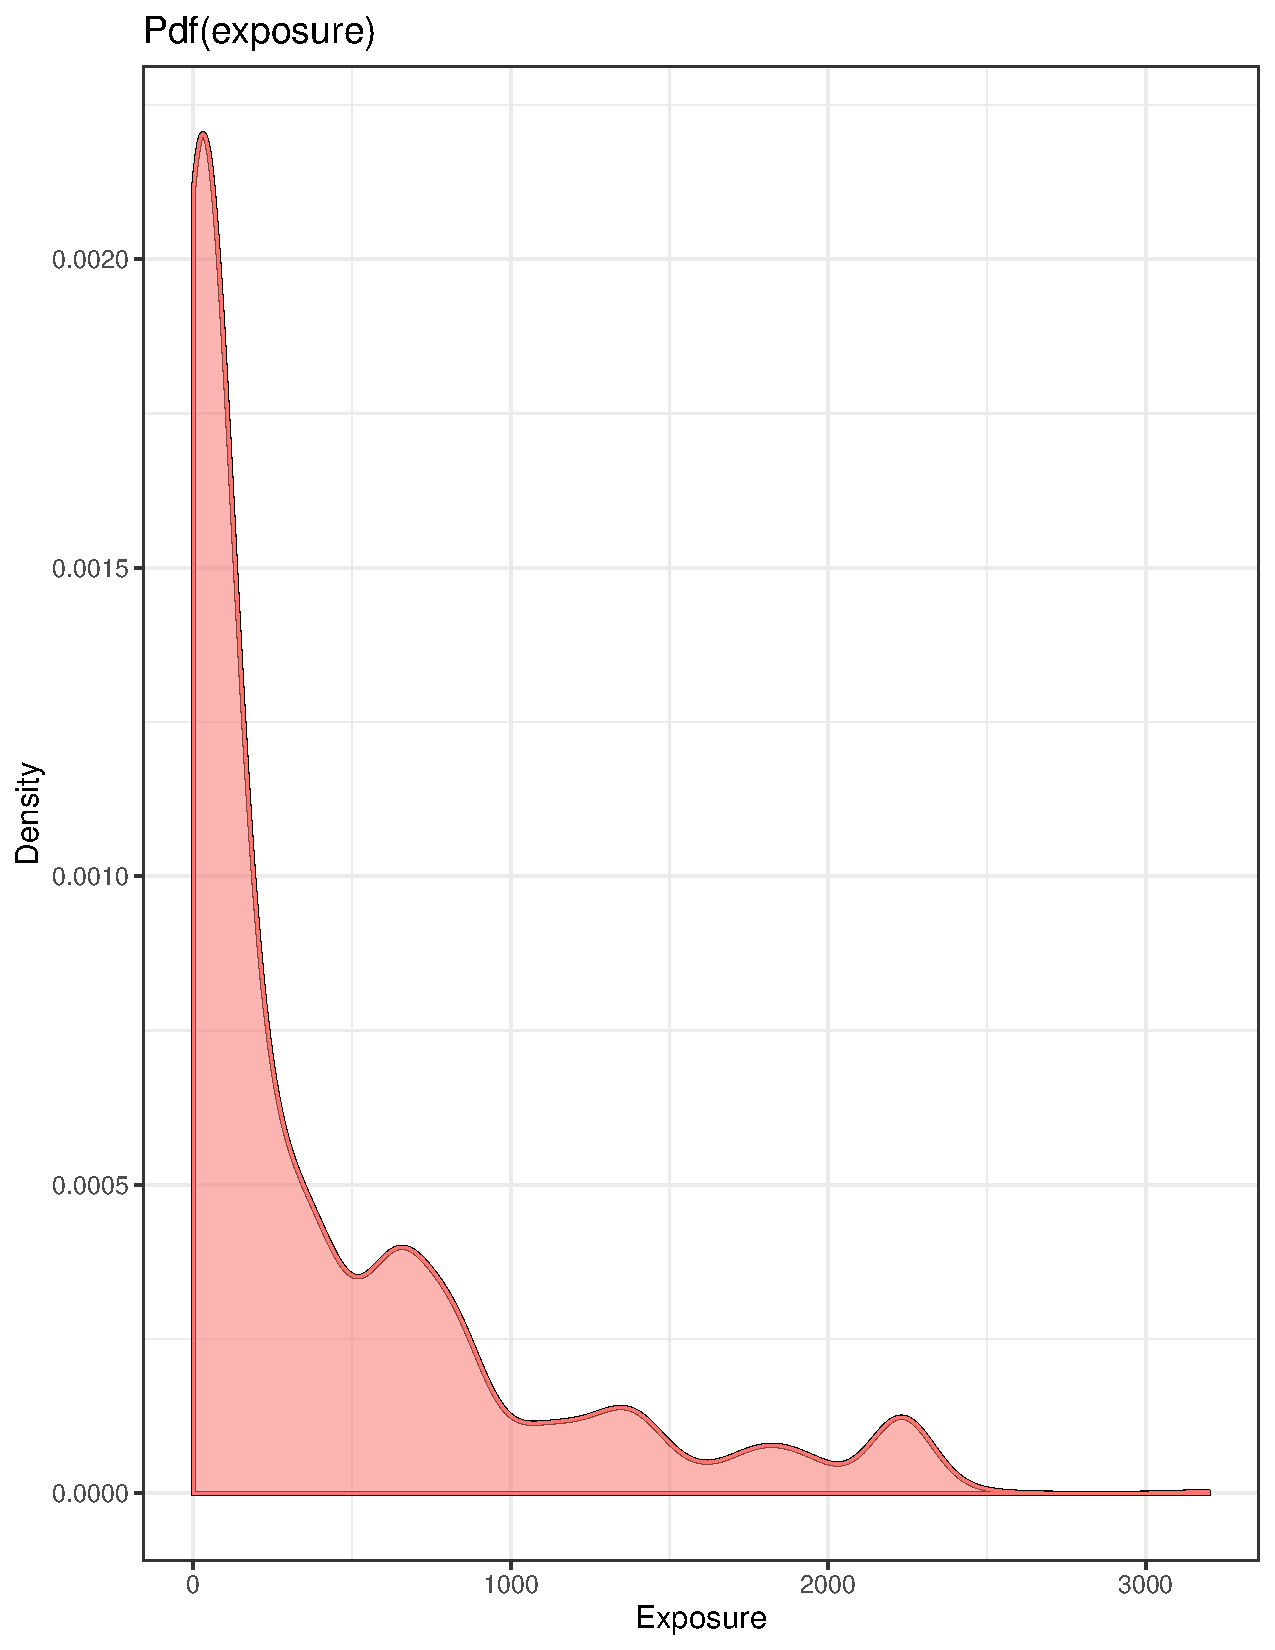
\includegraphics[height=7.5cm, width=5cm]{Exposure_cdf.pdf}
         &
         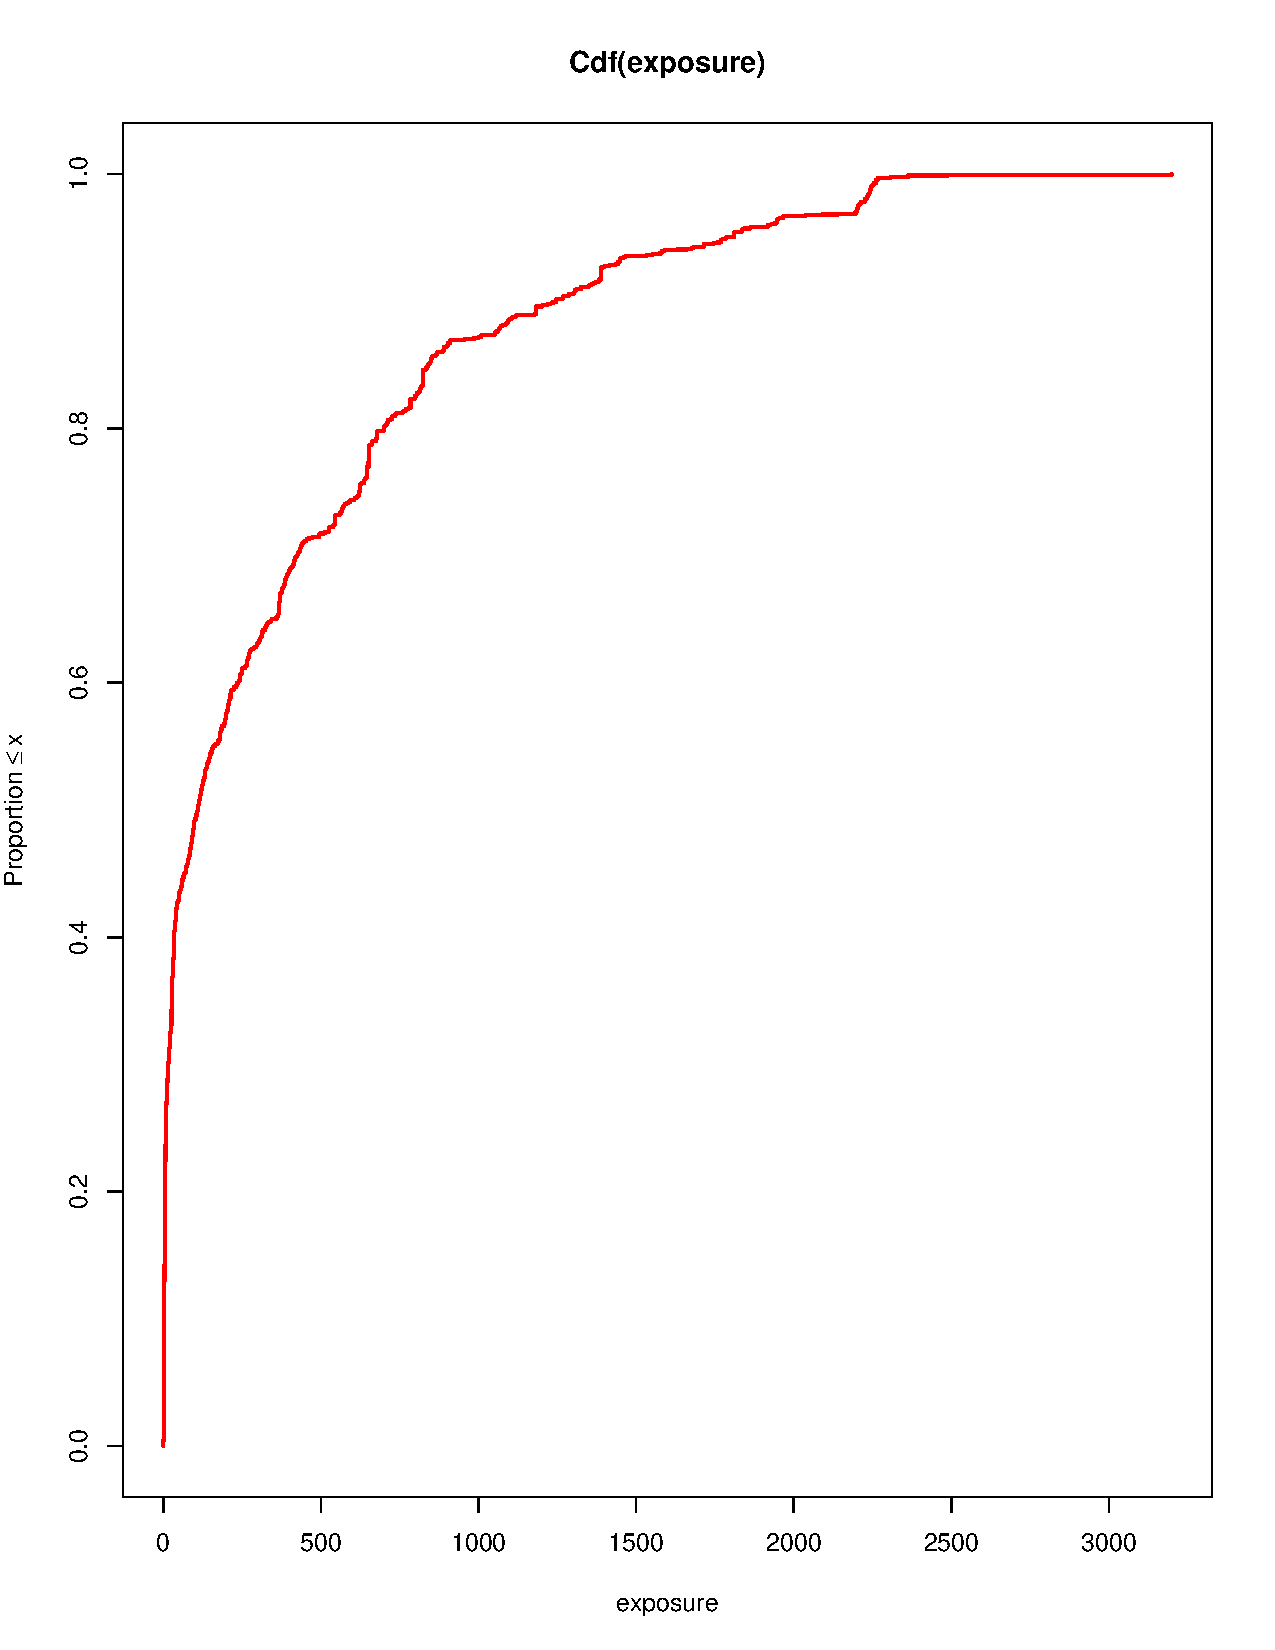
\includegraphics[height=7.5cm, width=5cm]{Dist_exposure.pdf}
         &
         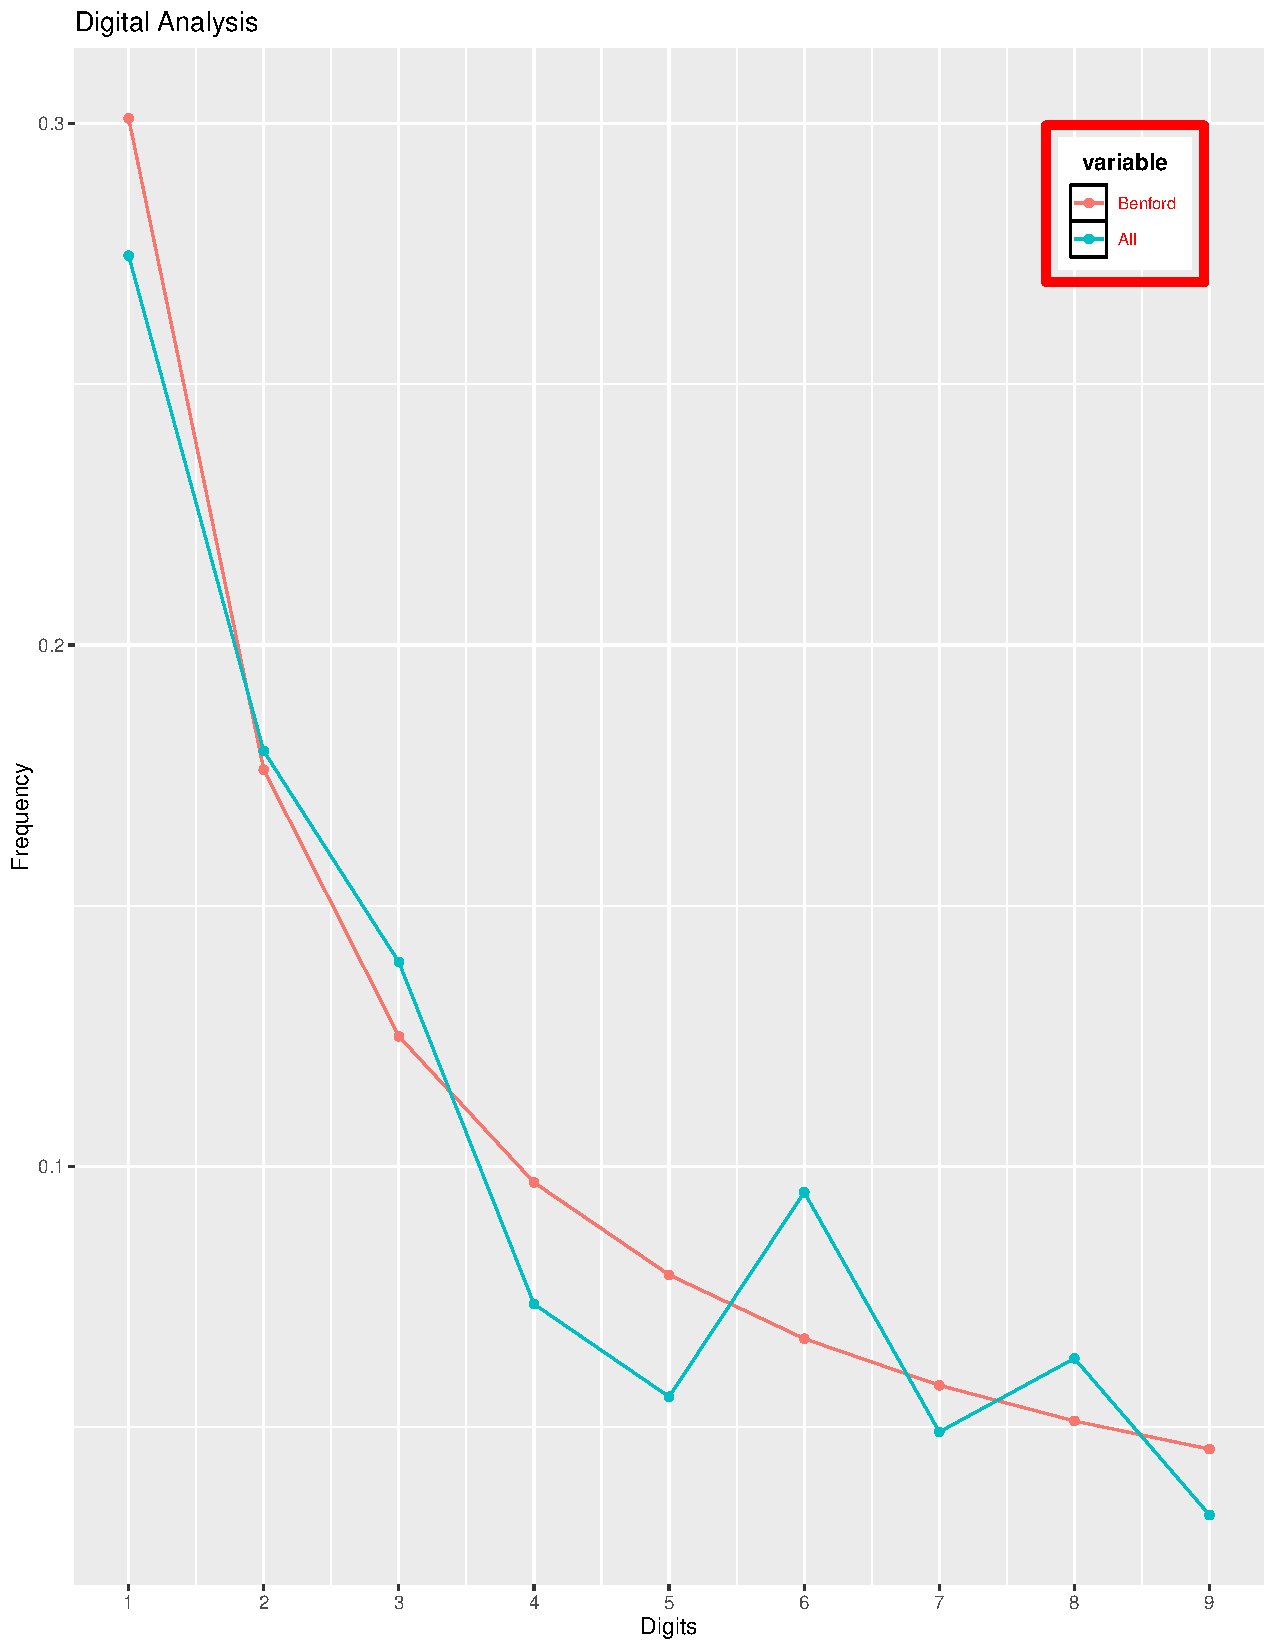
\includegraphics[height=7.5cm, width=5cm]{Benford.pdf}
         \end{tabular}
    \end{frame}
        \captionof{figure}{A simple comparison of the Sigmoidal like features of the fat-tailed, right skewed distribution for the Exposure variable, and first-digit analysis of frequency distribution from the exposure data with the expected distribution according to Benford's Law}
    \label{Exploration_analysis_exposure}
\end{figure}

The variable follows a logistic trend on \([0,1]\), implying an FIs
operational risk portfolio rises like a sigmoid function throughout the
period of observation, typically starting from \(0\), which then
observes a plateau in growth. The average exposure is 389.99 or about 1
year.\medskip

Grid plots \ref{Exploration_analysis_exposure} portray the logistic
function, together with a simple comparison of first-digit frequency
distribution analysis, according to Benford's Law, with exposure data
distribution. The close fitting nature implies the data are uniformly
distributed across several orders of magnitude, especially within the 1
year period.\medskip

\subsection{Characteristics of the covariates}

The characteristics of the operational risk portfolio are given by the
following covariates: \emph{UpdatedDay}, \emph{UpdatedTime} - the day of
the month and time of day the OpRisk incident occurs respectively;
\emph{TradedDay}, \emph{TradedTime} - the day in the month and time of
day the deal was originated respectively; The \emph{LossIndicator} as
indicated before is a binary variable consisting of two values: A \(0\),
which indicates pending or near misses, and \(1\), if the incident
results in a realised loss, meaning that there is significant p\&L
impact due to the OpRisk incident.\medskip

the \emph{Desk} is the location in the portfolio tree the incident
originated, it is a factor variable conisting of 10 categories;
\emph{CapturedBy}, the designated analyst who actions the incident, a
factor variable consisting of 5 categories; \emph{TraderId}, the trader
who originates the deal, a factor variable with 7 categories;
\emph{TradeStatus}, the live status of the deal, a factor variable with
4 categories; \emph{Instrument}, the type of deal, a factor variable
with 23 categories; \emph{Reason}, a description of the cause of the
OpRisk incident, a factor variable with 19 levels;
\emph{EventTypeCategoryLevel}, 7 OpRisk event types as per
@risk2001supporting, a factor variable with 5 categories;
\emph{BusinessLineLevel}, 8 OpRisk business lines as per
@risk2001supporting, a factor variable with 8 categories.\medskip

\singlespacing

\doublespacing

The continuous numerical variable \emph{Loss}, shows the financial
impact (severity) of the OpRisk incident in Rands. For the most part
(i.e.~96.1\% of the time) OpRisk incidents result in pending losses
and/or near misses, most realised losses (2.3\%) lie within the
{[}\textbf{R$200,00$}, \textbf{R$300,000$}{]} range. In the current
portfolio there are also five p\&L impacts higher than
\textbf{R$2.5$ million}.\medskip

\subsection{Characteristics of daily operational activity}

The distribution of daily losses and/or pending/near misses by
operational activities are represented in
\ref{Exploratory_Time_Day_Frequency3plot}. Figure
\ref{Exploratory_UpdateTime_Frequency3plot} shows that most operational
events occur in times leading up to midday (i.e.~10:50AM to 11:50AM),
the observed median is 11:39AM, and of these potential loss events, most
realised losses occur closest to mid-day. The frequencies of the loss
incidents in the analysed portfolio sharply decreases during the
following period, i.e.~from 12:10PM to 13:10PM, during which the least
realised losses occur.\medskip

Figure \ref{Exploratory_UpdateDay_Frequency3plot} shows that operational
activity increases in intensity in the days leading up to the middle of
the month, i.e.~\(10^{th}\) - \(15^{th}\); the observed mean is
\(14.49\) days, and of these potential loss events, realised losses
especially impact on the portfolio during these days.

\singlespacing

\doublespacing

\begin{figure}
\centering
\begin{subfigure}
   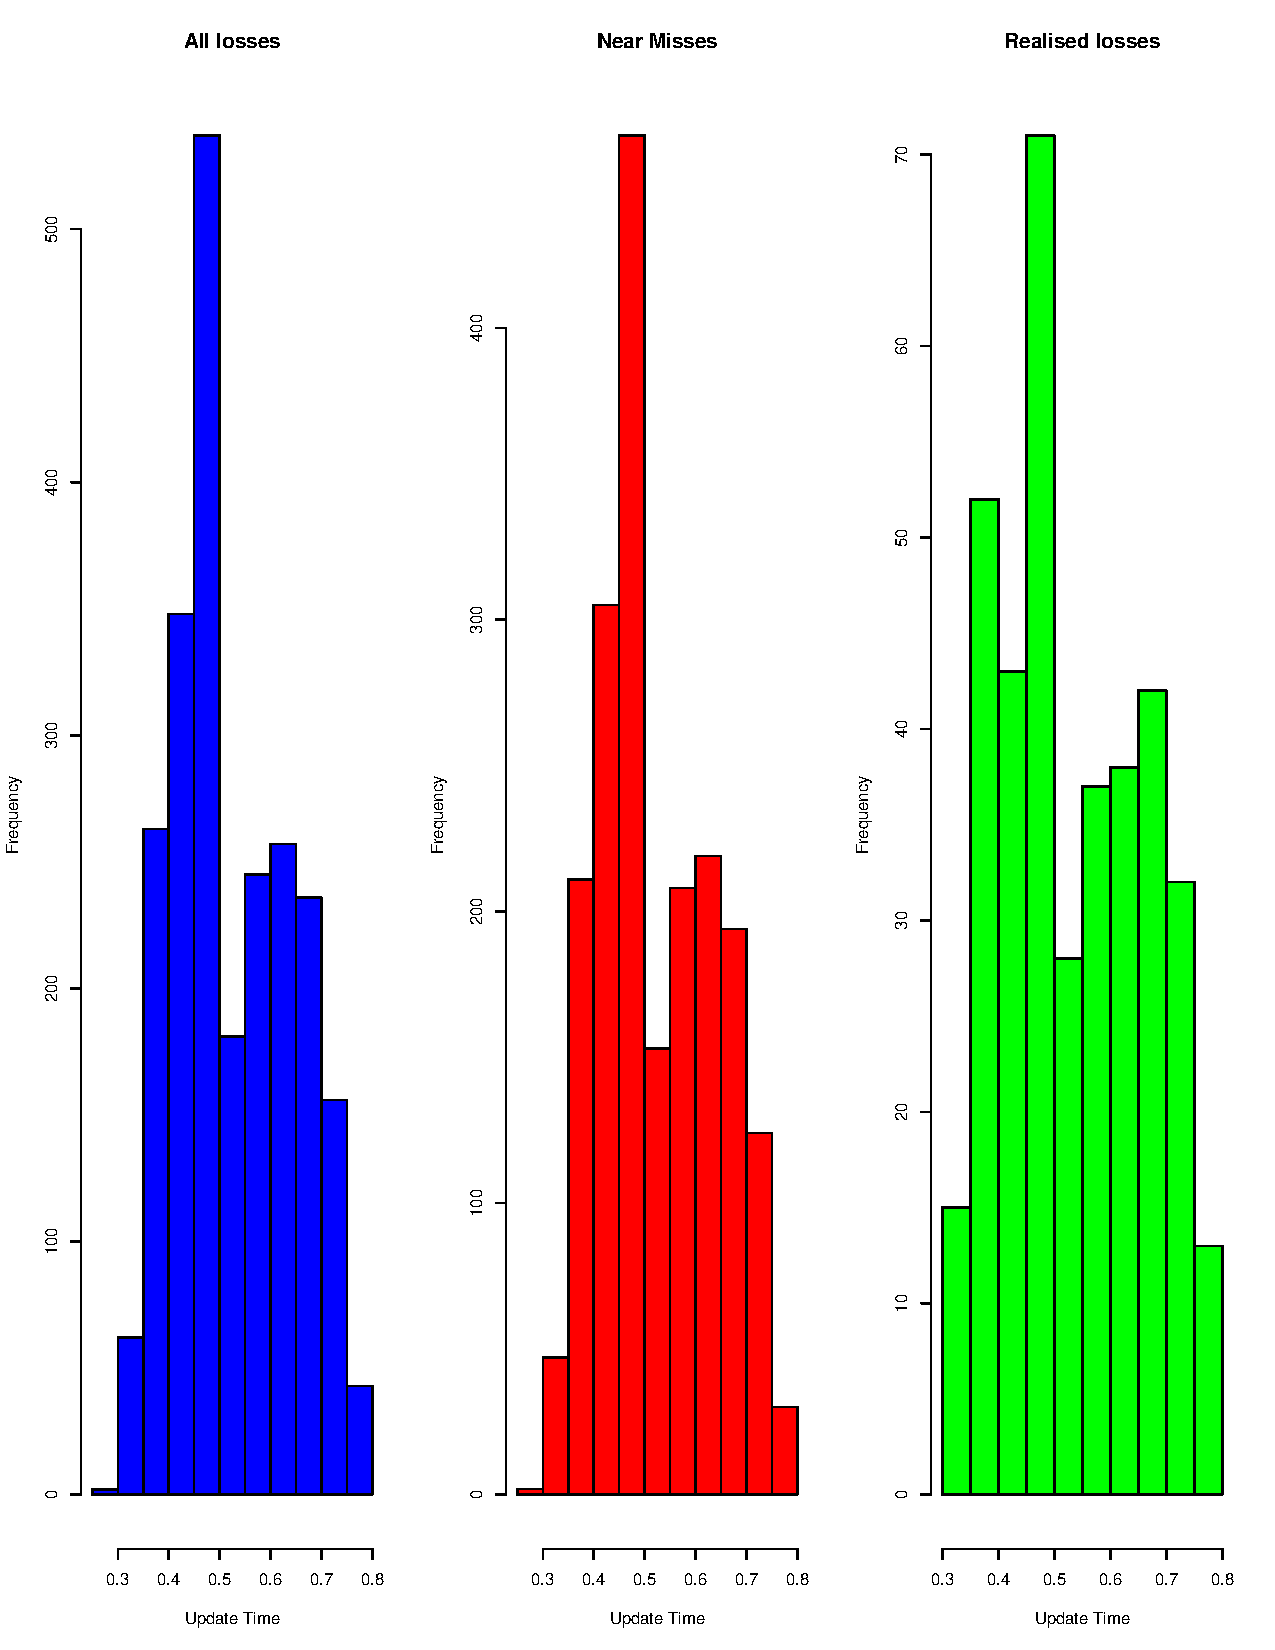
\includegraphics[height=7.5cm, width=15cm]{Exploratory_UpdateTime_Frequency3plot.pdf}
   \subcaption{Frequency distributions of operational incidents by the time in the day}
   \label{Exploratory_UpdateTime_Frequency3plot} 
\end{subfigure}

\begin{subfigure}
   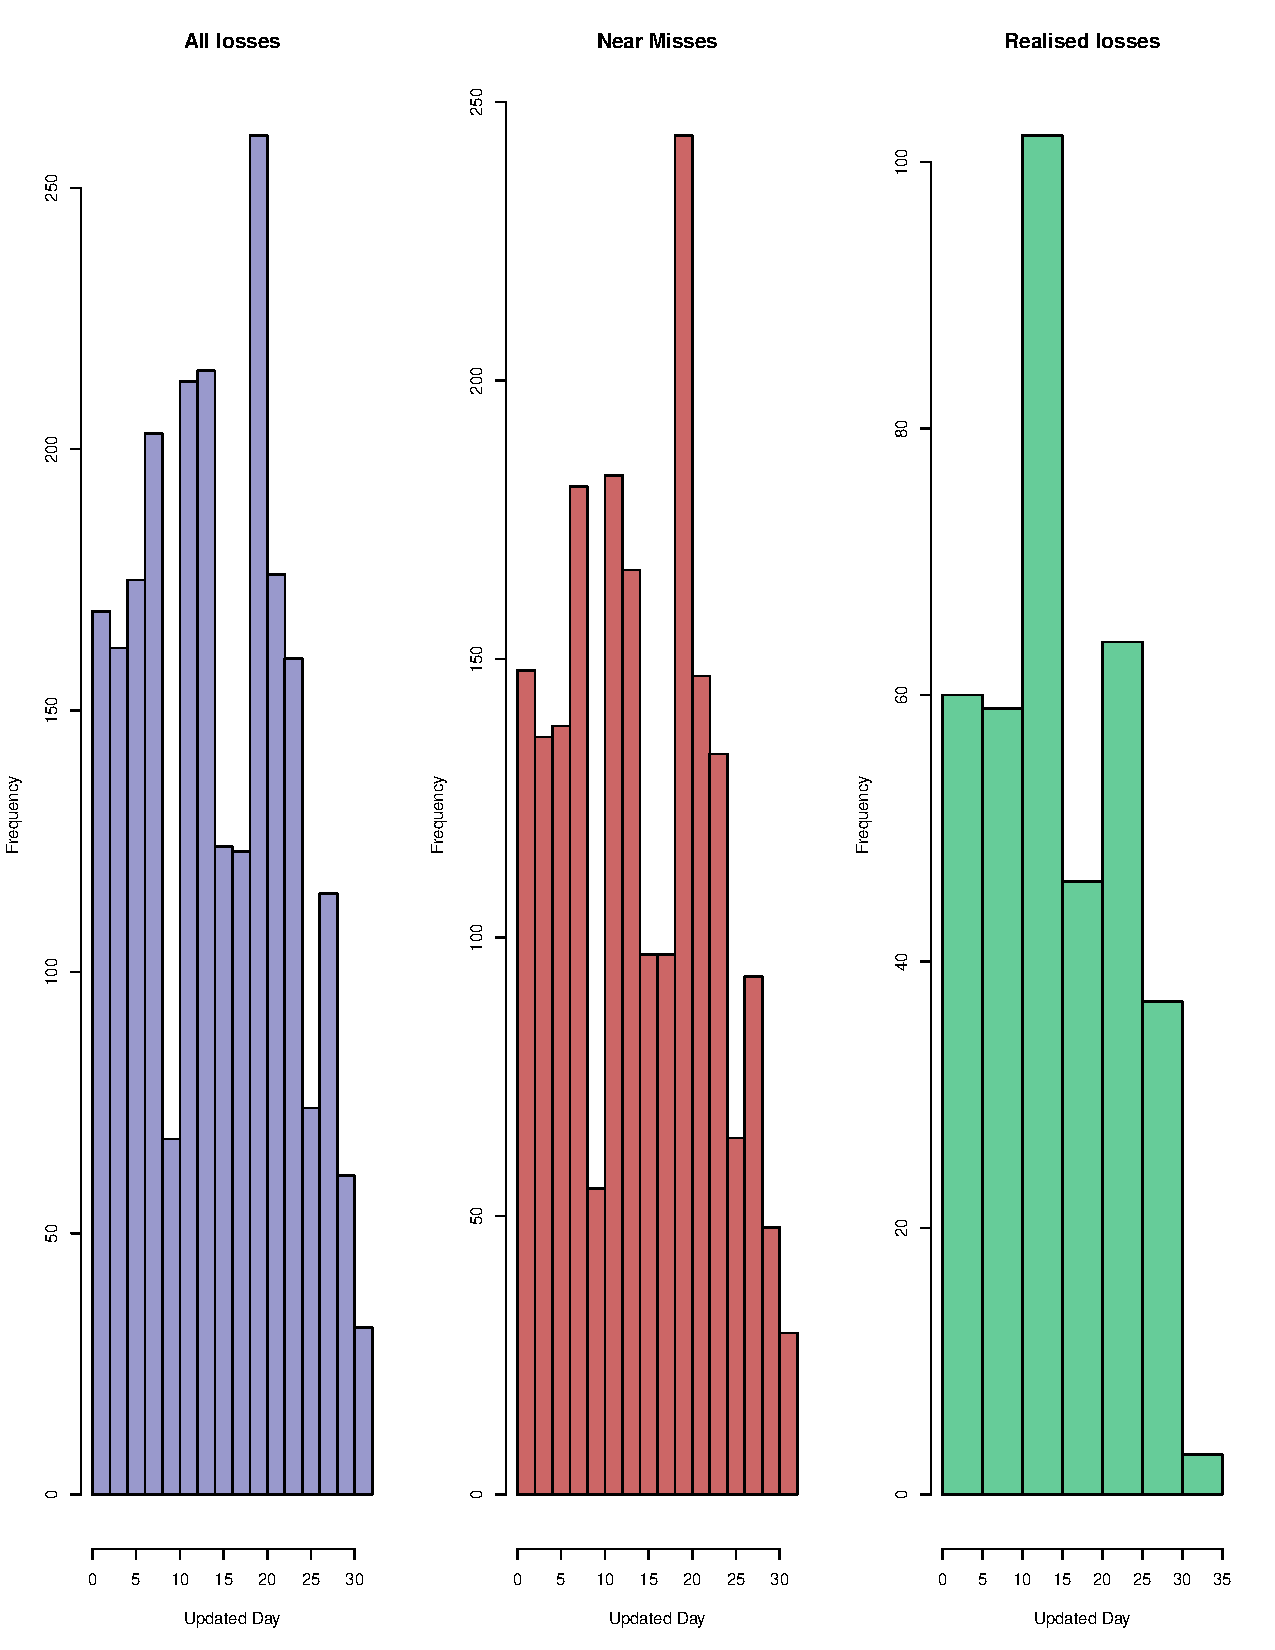
\includegraphics[height=7.5cm, width=15cm]{Exploratory_UpdateDay_Frequency3plot.pdf}
   \subcaption{Frequency distributions of operational incidents by the day in the month}
   \label{Exploratory_UpdateDay_Frequency3plot}
\end{subfigure}

\caption[Two numerical solutions: Histograms showing the distribution of UpdatedTime \& UpdatedDay by LossIndicator.]{The frequency distributions of All the losses, the realised losses, and pending/near misses of operational incidents by the day in the month when the indidents' occurred}
\label{Exploratory_Time_Day_Frequency3plot}
\end{figure}

Similarly, the influence of trading desk's on the frequency of
operational events can be analysed on the basis of the portfolio's
bidimensional distribution by variables \emph{Desk} and
\emph{LossIndicator}, which shows the proportions realised losses vs
pending and/or near misses for each particular desk. The bidimensional
distribution of \emph{Desk} and \emph{LossIndicator} is presented in a
contingency table, Table \ref{tab_Desk_Prop}, in which it's considered
useful to calculate proportions for each desk category.

\begin{figure}
\centering
\includegraphics[width=15cm,height=5cm]{Density_UpdateDay_TradedDay.eps}
\caption[Density plots showing a comparison of realised vs pending losses and/near misses over a month for the day in the month the OpRisk incident was updated to the day in the month trades were traded/booked]{Density plots showing a comparison of realised vs pending losses and/near misses over a month for the day in the month the OpRisk incident was updated to the day in the month trades were traded/booked}
\label{Density_Proportions}
\end{figure}

\singlespacing

\doublespacing

\begin{table}[ht]
\centering
\caption{Occurence of realised losses: proportions on desk categories}
\begin{tabular}{lccr}
\toprule
  & \multicolumn{3}{c}{No. of transactions} \\
Desk   & no Loss   & Loss & Total\\ 
\midrule
  Africa            &  49 & 10 &  59 \\
  Bonds/Repos       & 113 & 31 & 144 \\
  Commodities       & 282 & 45 & 327 \\
  Derivatives       & 205 & 24 & 229 \\
  Equity            & 269 & 66 & 335 \\
  Management/Other  &  41 &  2 &  43 \\
  Money Market      & 169 & 52 & 221 \\
  Prime Services    & 220 & 62 & 282 \\
  Rates             & 336 & 53 & 389 \\
  Structured Notes  & 275 & 26 & 301 \\
 \bottomrule
\end{tabular}\label{tab_Desk_Prop}
\end{table}

Thus, as illustratred in figure \ref{Desk_Proportions}, from 23,5\%; the
highest proportion of realised losses per desk is the Money Market (MM)
desk, the figures are decreasing, followed by Prime Services (22\%);
Bonds/Repos (21,5\%); Equity (19,7\%); Africa (16,9\%); Commodities
(13,8\%); Rates (13,6\%); Derivatives (10,5\%); Structured Notes (SND)
(8.6\%), to the least proportion in the Management/Other, a category
where only 4,7\% of operations activities were realised as losses.

\singlespacing

\doublespacing

\begin{figure}
\centering
\includegraphics[width=15cm,height=5cm]{Exploratory_Desk_Proportions.eps}
\caption[Desk category by realised losses]{Histograms showing the proportions of realised losses vs all losses including pending and/or near misses by desk category}
\label{Desk_Proportions}
\end{figure}

This behaviour can be extended beyond the trading desk, as represented
in Figure \ref{Mosaic_Instr_Trd_Tec}, a mosaic plot grid presenting the
structure of the OpRisk portfolio by Instrument, TraderId, CapturedBy
\footnote{i.e. the type of financial instrument, the trader who originated the incident on the deal, and the role of the technical support personnel who is involved in the query resolution.}
and the operational losses.

\singlespacing

\doublespacing

\begin{figure}
\begin{frame}
      \centering
       \begin{tabular}{cc}
        \textbf{Type of instrument traded} & \textbf{Role identification} \\
        \includegraphics[width=7.5cm,height=15cm]{Single_Instr.eps}
         &
         \includegraphics[width=7.5cm,height=15cm]{Stacked_TrId_TechSup.eps}
         \end{tabular}
    \end{frame}
    \caption{Mosaic grid plots for the bidimensional distribution by traded instrument, the trader originating the operational event, and by the technical support personnel involved in query resolution, against the dummy variable showing if a realised loss was reported.}
    \label{Mosaic_Instr_Trd_Tec}
\end{figure}

One can notice that the width of the bars corresponding to the different
categories, i.e.~Instrument, TraderId, CapturedBy, is given by their
proportion in the sample. In particular, for the category `at least one
realised loss', in the top right mosaic of Figure
\ref{Mosaic_Instr_Trd_Tec} portrays a increase in ``riskiness'' trending
up from Associate to AMBA, Analyst, Vice Principal, Managing Director,
Director, up to the risky ATS category, which are automated trading
system generated trades.\medskip

Figure \ref{Mosaic_Instr_Trd_Tec} bottom right mosaic plot for technical
support personnel for the category `at least one realised loss',
portrays a downward trend, slowing in riskiness from Unauthorised User
downward to Tech Support, Mid Office, Prod Controller down to the least
risky Prod Accountant. This intepretation makes sense given unauthorised
users are more likely to make impactful operational errors, technical
support personnel would also be accountable for large impacts albiet for
contrasting reasons, they are mandated to perform these deal adjustments
which have unavoidable impacts associated with them, whereas the former
group are unauthorised to perform adjustments therefore may lack the
skill, or be criminally minded insiders acting on their own or in unison
to enable their underhanded practices and intentions without raising any
suspicion.\medskip   

\begin{table}[!htbp] \centering 
  \caption{Summary statistics for all losses as per Instrument type} 
  \label{Stargazer} 
\begin{tabular}{@{\extracolsep{5pt}}lccccccc} 
\\[-1.8ex]\hline 
\hline \\[-1.8ex] 
Statistic & \multicolumn{1}{c}{N} & \multicolumn{1}{c}{Mean} & \multicolumn{1}{c}{St. Dev.} & \multicolumn{1}{c}{Min} & \multicolumn{1}{c}{Pctl(25)} & \multicolumn{1}{c}{Pctl(75)} & \multicolumn{1}{c}{Max} \\ 
\hline \\[-1.8ex] 
Mean & 23 & 34,603 & 46,007 & 306 & 7,697 & 44,157 & 192,513 \\ 
\hline \\[-1.8ex] 
\end{tabular} 
\end{table}

In another mosaic plot, Figure \ref{Mosaic_Contingency}, the
bidimensional distribution of transactions by trader and realised vs
pending losses, conditional on the trade status is presented and
analysed. Here, and in the contingency table, Table
\ref{tab:Mosaic_Contingency}, we can clearly see the following trends:
In BO-BO confirmed status - an increase in realised losses from the
leftmost TraderID (i.e.~AMBA) to right, and the opposite for
transactions performed in BO Confirmed status (both with two
exceptions). In particular, the biggest number of realised losses in
both BO and BO-BO Confirmed statuses occur due to automated trading
systems (ATS) who also give rise to the exceptions mentioned.\medskip

\singlespacing

\singlespacing
\begin{figure}
\centering
\textbf{Mosasic plot for trader identification and loss indicator, by trade status}
\includegraphics[width=\linewidth,height=0.75\linewidth]{Mosaic_Contingency.eps}
\caption[Portfolio structure by trader, trade status and number of realised losses]{A mosaic plot representing the structure of the operational risk portfolio by trader identification (TraderId), the status ofthe trade (TradeStatus) and the number of realised losses vs pending or near misses}
\label{Mosaic_Contingency}
\end{figure}
\doublespacing

Table \ref{tab:Crosstab_covariate} presents the most frequent category
in the operational risk dataset for each possible covariate.

\begin{table}[htbp]
        \centering
        \textbf{Crosstab of trader identification and loss indicator, by trade status}
\singlespacing        
        \small
        \setlength\tabcolsep{2pt}
            \begin{tabular}{|p{2cm}|p{2cm}|l|l|l|l|l|l|p{2cm}|p{2cm}|} \hline
            & & \multicolumn{7}{|c|}{Trader Identification} \\ \hline
            TradeStatus & Loss Indicator & Amba & Analyst & Associate & ATS & Director & Mng Director & Vice Principal \\\hline
            \multirow{2}{*}{BO-BO Confirmed} & 0 & 24 & 136 & 320 & 0 & 282 & 52 & 49 \\ \cline{2-9}
                                   & 1 & 2  &  15 & 43 & 0 & 50 & 18 & 16 \\\cline{2-9}
            \multirow{2}{*}{BO Confirmed} & 0 & 17  & 299 & 153 & 13 & 257 & 102 & 153 \\ \cline{2-9}
                                   & 1 &  3 &  71 & 12 & 8 &  62 & 23 & 30 \\ \cline{2-9}
            \multirow{2}{*}{Terminated}       & 0 & 83 & 9 & 1 & 0 & 0 & 2 & 1 \\ \cline{2-9}
                                  & 1 & 17 & 1 & 0 & 0 & 0 & 0 & 0 \\ \cline{2-9}
            \multirow{2}{*}{Terminated/Void}  & 0 & 2 & 0 & 0 & 0 & 2 & 1 & 1 \\ \cline{2-9}
                                   & 1 & 0 & 0 & 0 & 0 & 0 & 0 & 0 \\ \hline
            \end{tabular}
            \caption{A contingency table showing the bidimensional distribution of transactions by trader identification vs realised and/or pending losses, conditional on the trade status}
            \label{tab:Crosstab_covariate}
\end{table}
\doublespacing

\begin{table}[htbp]
        \centering
        \textbf{Modal classes for the categorical variables} 
\singlespacing        
        \small
        \setlength\tabcolsep{2pt}
            \begin{tabular}{|l|l|p{4cm}|} \hline
            Variable & Modal class or category & Name of modal class \\\hline
            Desk & Rates & DeskRates \\ \cline{1-3}
            CapturedBy & TECHSUPPORT & CapturedBy\_TECHSUPPORT \\ \cline{1-3}
            TradeStatus & BO confirmed & TradeStatus\_BO confirmed \\ \cline{1-3}
            TraderId & DIRECTOR & TraderId\_DIRECTOR \\ \cline{1-3}
            Instrument & Swap & Instrument\_Swap \\ \cline{1-3}
            Reason & Trade enrichment for system flow  & Reason\_Trade enrichment for system flow \\ \cline{1-3}
            EventTypeCategoryLevel & EL7 & EventTypeCategoryLevel\_EL7 \\ \cline{1-3}
            BusinessLineLevel & BL2 & BusinessLineLevel\_BL2 \\ \cline{1-3} 
            \end{tabular}
            \caption{A contingency table showing the bidimensional distribution of transactions by trader identification vs realised and/or pending losses, conditional on the trade status}
            \label{tab:Mosaic_Contingency}
\end{table}
\doublespacing

\singlespacing

\end{document}
